%! TeX root = main.tex
\documentclass[conference]{IEEEtran} \IEEEoverridecommandlockouts
% The preceding line is only needed to identify funding in the first footnote.
% If that is unneeded, please comment it out.
%Template version as of 6/27/2024

\usepackage{cite} \usepackage{amsmath,amssymb,amsfonts}
\usepackage{algorithmic} \usepackage{graphicx} \usepackage{textcomp}
\usepackage{xcolor} \def\BibTeX{{\rm B\kern-.05em{\sc i\kern-.025em
b}\kern-.08em T\kern-.1667em\lower.7ex\hbox{E}\kern-.125emX}} 

\title{Autonomous Firewalling: Autowall\\}

\author{\IEEEauthorblockN{Alvin Leung} \IEEEauthorblockA{\textit{Computer
Science and Engineering} \\ \textit{Univerisity of Nevada, Reno}\\ Reno, United
States of America \\ aleung@unr.edu} }

\begin{document}

\maketitle

\begin{abstract} Due to the rise of cybercrime, industries
	and consumers have begun to worry about their electronic device security and the possibility of device compromise
	. This has led to
	a majority of industries and homes to begin using
	intrusion detection systems (IDS) to discover attacks. There are many popular open source options for IDS, however,  
	perhaps the most popular is SNORT. Many enterprises use SNORT as it is free and flexible for many industries
	through its custom rule-writing capability.
	and provides enterprise and
	home users with an easy option to safely encrypt and decrypt their files, discouraging
	data theft. Thus, BitLocker disks are becoming more and more common in
	both law enforcement and digital forensic fields. However, likewise, accidental partition deletion with
	BitLocker is also just as common. Whether accidental or intentional, 
	data recovery has become complicated, especially with BitLocker. 
	With a BitLocker disk, standard troubleshooting and data recovery techniques are not 
	sufficient due to BitLocker encrypting the data into an unreadable format
	that no human nor software can read without a decryption key. However, BitSaver is a new command-line interface (CLI) program that
	detects and finds BitLocker partitions and rebuilds partition tables to
allow an encrypted disk to be readable again, assuming that a BitLocker
recovery key exists and is in the possession of law enforcement or data
forensics. \end{abstract}

\begin{IEEEkeywords} encryption, data, forensics, BitLocker, recovery.
\end{IEEEkeywords}

\section{Introduction}

\subsection{BitLocker and Digital Forensics} BitLocker is an application that
is very relevant in the field of Information Technology (IT) and digital
forensics. Most enterprises have policies that allow their systems to
automatically and routinely encrypt data. On top of this, the enterprise may even
recycle keys monthly to further protect data. This is to prevent confidential
data from being stolen. However, this often creates new barriers for digital
forensics teams when they need to analyze a disk for official reason such as
law enforcement. According to North Forensics, encryption makes data unreadable
without a key, bypassing even the most advanced forensic tools. Thus, BitLocker becomes a
time-consuming, unavoidable, and complex process for data forensic technicians to overcome, oftentimes
impossible without sophisticated tools and procedures.

On top of this, the legal aspects of evidence that utilizes encryption can be
complicated. Meticulous documentation is required to maintain integrity of an
encrypted piece of evidence so that it can be used in the court of law \cite{b5}.

\subsection{BitSaver Objectives and Motivation} When an individual manually
deletes a BitLocker partition, the data does not get deleted. Instead, the disk
marks the partition as unallocated space so that new data can be written to the unallocated partition.
Thus, the data remains on the drive so long as no additional data overwrites the previous data.
However, the data partition still cannot be read directly, either with or without data recovery software,
due to the encryption from BitLocker. Suspects who are
informed on disk partitioning schemes and BitLocker may delete a BitLocker partition in order
to stall law enforcement or obscure any evidence that a disk might contain. This leads to law enforcement
being unable to use standard data recovery procedures.

The goal of this project, BitSaver, is to create a tool that can automate the recovery of
BitLocker partitions that have been deallocated into unallocated space on a disk.
Usually, deallocated space naturally occurs when a storage device has not been used or formatted prior.
However, it can also occur when an individual manually deletes disk partitions such
as with the Windows built-in DiskPart tool. BitSaver is focused on creating a tool that works for
Windows as the Windows operating system is the primary operating system that utilizes BitLocker. Thus,
BitSaver does not work for other operating systems like MacOS or Linux/UNIX and will not work even in
future versions.

In general, law enforcement, digital forensics, and enterprise IT technicians will be able
to use this application to recover BitLocker partitions that have been deleted
and not formatted (and not overwritten). For example, if a suspect knows that law enforcement is on
their "trail", the suspect may delete BitLocker partitions and not format the
deleted partitions of their devices to obscure the data but still be able to potentially recover
the data at a later point (post-investigation). The suspect would still need to
hide their recovery keys, but a barrier to the potentially vital information has formed for law
enforcement. Another example would be if a trainee IT technician accidentally
deleted a BitLocker partition on an important, critical data drive while trying
to install the Windows operating system for another disk or partition. In these cases,
law enforcement and the IT technician would have a way of potentially restoring the otherwise unrecoverable data.
Of course, there are already
many techniques for rewriting boot records to restore functionality. However,
most tools require the user to perform potentially destructive disk writes,
which can potentially cause permanent data loss. This is where the application can be very
useful. BitSaver automatically detects and locates BitLocker partitions,
accurately calculates partition sizes, and safely writes boot records for its users to avoid dangerous writes.


\subsection{BitSaver Plans and Implementation} To implement this tool, standard
Python libraries, PowerShell commands, and Runtime Software's open source, free
DriveDoppel executable were all used \cite{b7}. Python was chosen to implement a user-friendly
interface to communicate with the user and to wrap special system calls. Standard libraries like Hashlib, 
Ctypes, etc. were used for their ability to analyze disk data and make calls to the Windows operating system.
Non-standard libraries include: pyuac, pypiwin32, PySide6, and hexdump. PowerShell was used to communicate system calls to the disk safely in Windows.
Lastly, DriveDoppel was used to safely write boot records to a disk.

When ran, the program will open up an interface that allows users to select
numbers representing the user's choices. Initially, the program will collect information about all storage devices
detected on the system, including internal and external storage devices.
Afterwards, the device will allow users to perform operations on disks such as
selecting disk, hexdumping BitLocker sectors, reading the boot sector, and repairing BitLocker master boot
records. The system is also intentionally configured to stop users from selecting the boot
drive as an option to prevent critical damage on the operating system running the program. A depiction of
the menu is shown in Fig.~\ref{fig:menu}. Users in this screen are able to see
the hostname of the machine they are working on and see many useful, surface-level attributes
about the storage devices connected to the machine such as drive number, friendly 
drive names (official models, which are useful for documentation purposes), encryption status, and capacity.

\begin{figure}[t] \centering 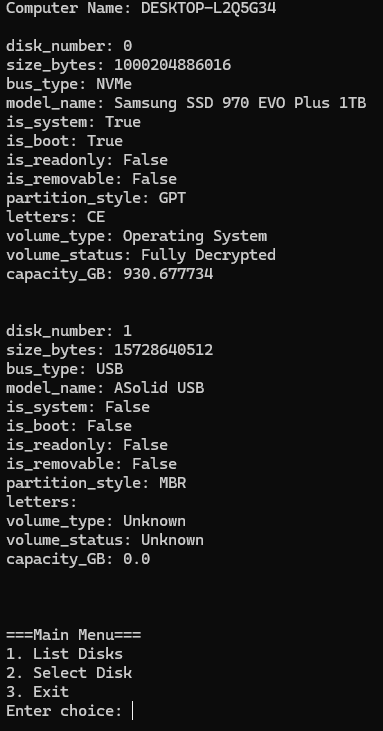
\includegraphics[width=\columnwidth]{menu.png}
\caption{BitSaver CLI for users to choose options.} \label{fig:menu}
\end{figure}

\section{Challenges and Threat Models} \subsection{Commerical BitLocker Restoration Software}
Restoring deleted BitLocker partitions is not a rare troubleshooting issue. In fact, there are many online sources
that provide methods to resolve such issues such as those from M3 Software or
EaseUS \cite{b3,b4}. These sources all describe the relatable issue of accidentally deleting BitLocker partitions.
However, almost every single one of these sources
do not provide systematic command calls or low-level steps to resolve the
issue.

Instead, almost every source provides their own sponsored, paid software to
resolve this issue. On the other hand, BitSaver believes that potential critical data loss should
not be left to the mercy of paid tools. Instead, BitSaver seeks to provide the
foundation of open source software that can be used to protect and restore critical data for free.

\subsection{Manual Processes}

There are several sources that provide manual steps to resolve this issue, which
this entire project is based on. For example, Norman Bauer published a blog
page in 2013 that instructs people on how to restore a deleted BitLocker partition using
only the Windows OS and the open source 7-zip application. However, his methods
merely takes a copy of the data off of a drive rather than
restore the drive's original BitLocker functionality, which may have different legal
implications due to evidence validity. BitSaver intends to restore a drive's
BitLocker functionality without destroying the data \cite{b2}.

Another source, which provides the groundwork for this application, is Runtime
Software's BitLocker data recovery guide. The guide instructs the user on how to
explore a disk's sectors in order to map out and restore the affected partition 
using DiskExplorer X, DriveDoppel, and GetDataBack Pro.
While the content is very well-written, the guide still attempts to sell its
paid software GetDataBack Pro. However, its freeware DiskExplorer X was used in
this project to verify the integrity of each step taken by the application in
order to make sure that the application is performing correct computations and searches \cite{b6}.
Furthermore, DriveDoppel is directly used in the program for the accurate MBR
writes. Lastly, GetDataBack Pro was used to verify the inaccessibility of
the data stored on deleted, locked BitLocker partitions \cite{b1}.

\section{Related Works} 

\subsection{Gathering Disk Information} 

To start off, an easy and
reproduceable testing environment is created. In this environment, a small 16 GB USB drive was
used as the primary form of storage device in BitSaver's earliest tests. Due to the time it
takes to encrypt and decrypt large drives, larger drive sizes were not
considered for initial testing of functionality. The 16 GB USB drive was formatted to FAT32, and the
recovery key was stored externally for unlocking and verification. To begin, Windows's built-in
BitLocker application was used to encrypt the 16 GB USB drive as shown in
Fig.~\ref{fig:bitlockered_drive}.

\begin{figure}[t] \centering
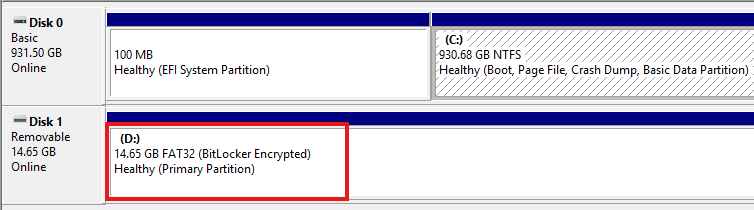
\includegraphics[width=\columnwidth]{bitlockered_disk.png} \caption{BitLocker
encrypts the 16 GB USB drive, and Windows recognizes the BitLocker properties
of the USB drive.} \label{fig:bitlockered_drive} \end{figure}

Afterwards, the disk's BitLocker partition was manually deleted via Windows DiskPart.
This resulted in Windows Disk Manager recognizing the partition as unallocated
as shown in Fig.~\ref{fig:delete_partition}. Accessing the data also prompts a
formatting request (which must not be accepted to prevent data loss) as shown
in Fig.~\ref{fig:inaccessible}. Standard data recovery software yields no
results when files are analyzed for recovery such as Get Data Back Pro (GDBP). 

\begin{figure}[t] \centering
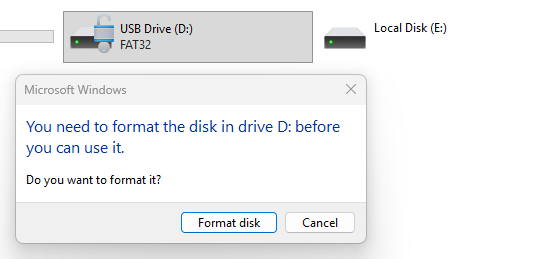
\includegraphics[width=\columnwidth]{inaccessible.png} \caption{DiskPart
operation renders the drive inaccessible, which prompts user to reformat the
disk.} \label{fig:inaccessible} \end{figure}

\begin{figure}[t] \centering
	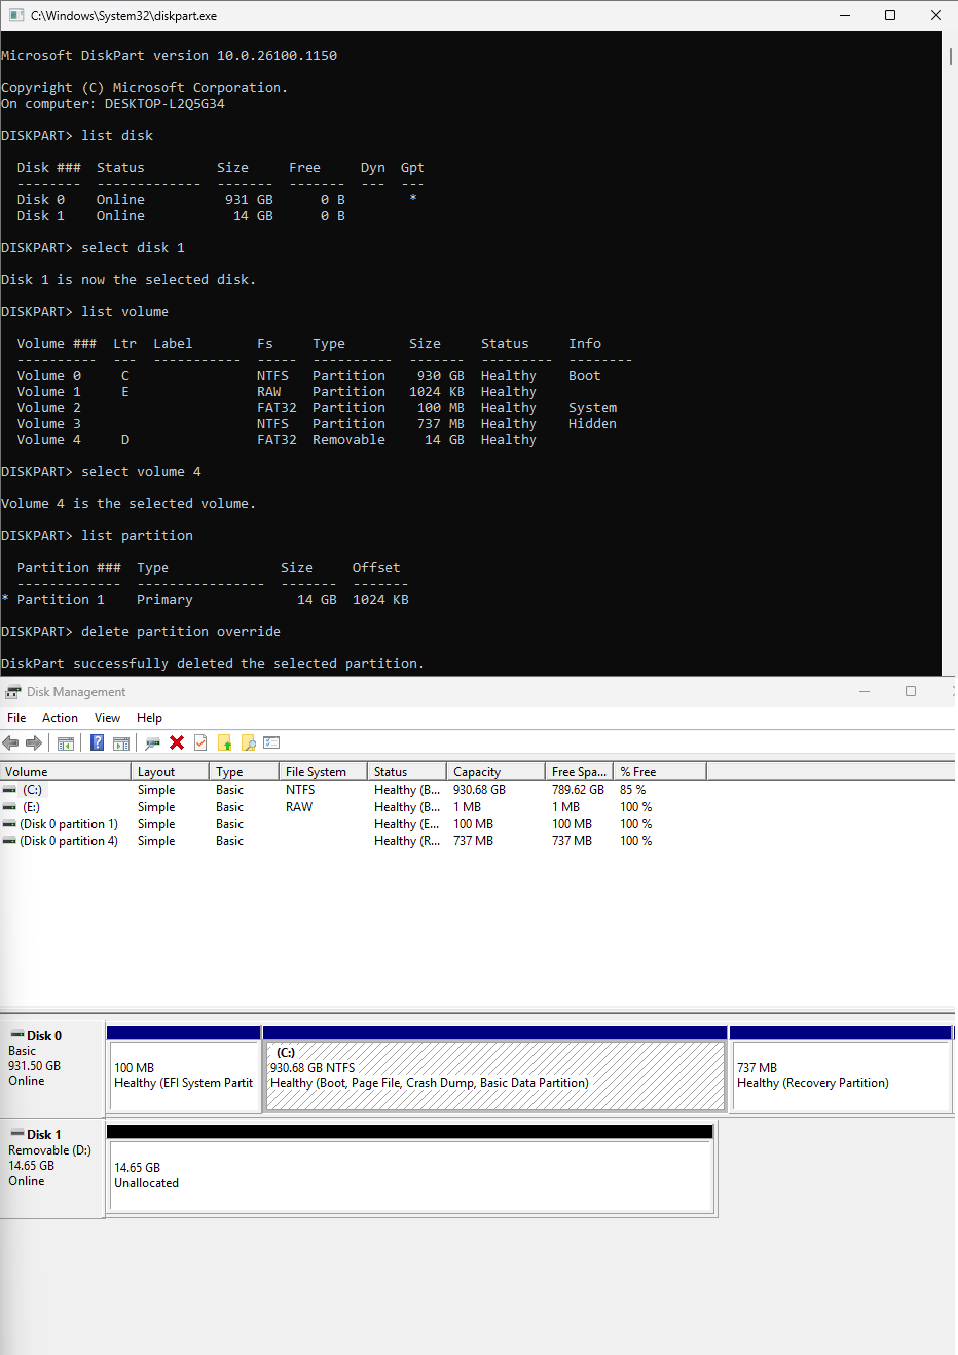
\includegraphics[width=\columnwidth]{delete_partition_new.png}
	\caption{DiskPart operation to forcefully delete BitLocker partition
	(Top). Disk becomes unallocated after deletion (Bottom).}
	\label{fig:delete_partition} \end{figure}

	When a partition deletion occurs, the disk's partition table has been
	modified to mark the deleted partition as unallocated. A rewrite of the boot
	record on the disk is required to restore functionality to the disk (essentially to
	undo the operation preceding the deletion.
	However, the boot record is incredibly sensitive and requires an
	accurate byte count of the size of the BitLocker partition to avoid
	deleting unintended data.

	Thus, the first step required is to gather the data of all storage devices to
	obtain information about the partitions on each disk. The program
	utilizes the Windows built-in PowerShell command Get-BitLockerVolume and
	Get-Disk to gather and format data regarding all data storage on the
	system. Some of the most important information gathered about the disks
	is the disk number, size, boot status, drive letters, and BitLocker
	status. All of this information is neccessary to perform accurate, informed disk
	operations.

	Afterwards, BitSaver marks the disk that the program is running off of as
	unprocessable and unselectable to protect the native boot drive from destructive disk
	writes. If selected, the program will error out and prompt user to
	choose a different disk. All other devices are allowed to be operated on.
	If a valid, non-boot device is selected, deeper disk information is gathered via
	the Windows Get-Disk function such as logical sector size, Logical Block Addressing
	(LBA) sector count, and true size. Logical sector size is the total
	size of a single sector measured in bytes. The LBA sector count is the
	number of logical sectors on the storage device. Lastly, the total size
	is the number of bytes that the device can hold. The LBA sector count
	can be calculated by the following:
 
	\begin{equation} s/l=\gamma\label{eq:lba_eq} \end{equation}

	where $s$ is the capacity of the storage device in bytes, $l$ is the
	logical sector size also in bytes, and $\gamma$ is the LBA sector count. The LBA
	sector count is crucial to performing correct disk operations as a disk is accurately divided
	by these sectors.

	\subsection{Finding BitLocker Sector and Count}

	Using the Equation~\ref{eq:lba_eq}, it becomes trivial to calculate the
	number of LBA sectors for the partition table parameters as shown in
	Fig.~\ref{fig:extra_parameters}. The next step is to calculate the
	start sector and the end count. The starting sector of all BitLocker partitions always has a hex
	pattern of "2D4656452D46532D". This is because all BitLocker partitions have the signature 
	"-FVE-FS-" \cite{b1}. The hex pattern is merely a conversion of the string "-FVE-FS-" in hex. 
	To find the starting sector of a
	BitLocker sector, BitSaver iterates from sector 0 (start of
	the physical disk) and finds the first iteration of the BitLocker signature in hex. In most
	cases, the BitLocker signature will be on sector 2048 as shown in
	Fig.~\ref{fig:bitlocker_sector}.

	\begin{figure}[t] \centering
		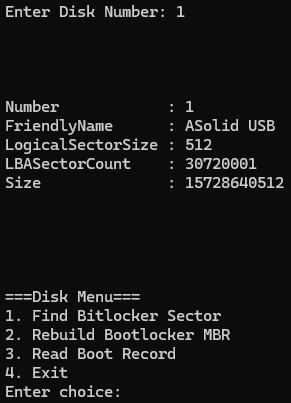
\includegraphics[width=\columnwidth]{extra_parameters.png}
		\caption{BitSaver calculates the logical sector size,
		LBA sector count, and size of the disk selected for disk
	operations.} \label{fig:extra_parameters} \end{figure}

	\begin{figure}[t] \centering
	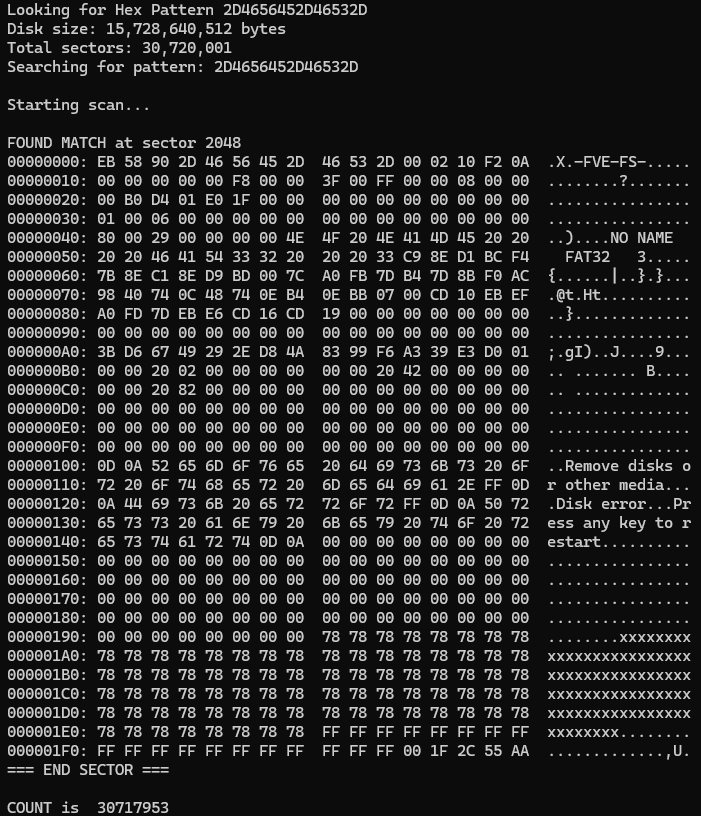
\includegraphics[width=\columnwidth]{bitlocker_sector.png} \caption{BitSaver 
		performs a hexdump of all sectors to look for the unique, BitLocker
signature.} \label{fig:bitlocker_sector} \end{figure}

Afterwards, the partition size needs to be calculated by the following:

\begin{equation} \gamma-b=p\label{eq:partition_size_eq} \end{equation}

where $\gamma$ is the LBA sector count of the storage device, $b$ is the starting
sector for the BitLocker partition, and $p$ is the partition size in sectors. This is used to calculate
the partition entry to write to the partition table in the next step. 

\subsection{Rebuilding the BitLocker MBR}

After choosing to rebuild the BitLocker MBR, the user is prompted for the file
system type of the expected drive as shown in
Fig.~\ref{fig:file_system_options}. Though this information is often not known,
in most cases, NTFS and FAT32 are safe choices for the Windows operating
system. After the file system is selected, the application will seek out the
BitLocker starting sector and the BitLocker partition size using the
aforementioned equations.

\begin{figure}[t] \centering
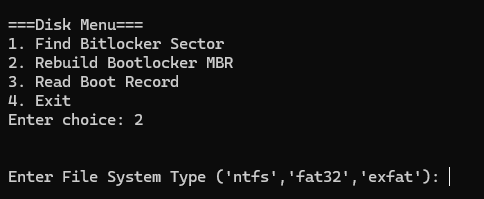
\includegraphics[width=\columnwidth]{file_system_options.png}
\caption{BitSaver prompts the user to enter the expected file system of the disk.}
\label{fig:file_system_options} \end{figure}

Afterwards, the application calls on DriveDoppel, a third-party executable used
for the sensitive disk operations. The application sends DriveDoppel its
parameters (the file system type, BitLocker starting sector, and partition
size) and runs the executable on the selected disk. The CLI notifies the user
of the potentially destructive operation.

If the user approves, DriveDoppel writes the new partition data to the partition
table as shown in Fig.~\ref{fig:disk_doppel}. With a correct write, Windows
should recognize the disk as having BitLocker enabled and prompt the user to
enter the recovery key for the disk (in some cases, a physical disconnect and reconnect may be needed
for Windows to recognize the change in the device's partition table). After entering the correct recovery key, the user should
be able to access the data previously locked anyway by BitLocker and
unallocated partitions as shown in Fig.~\ref{fig:accessible_again}.


\begin{figure}[t] \centering
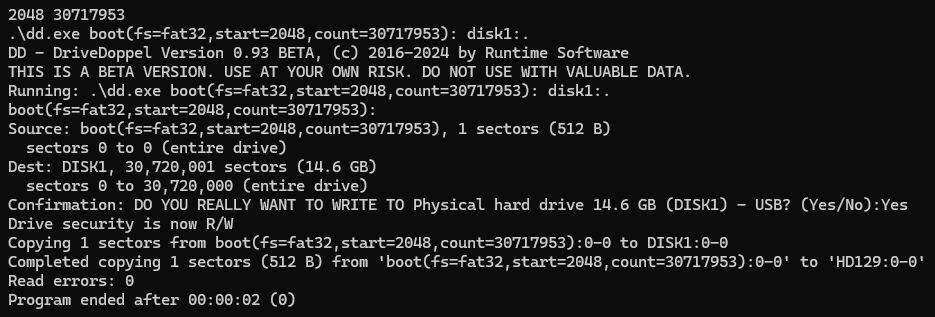
\includegraphics[width=\columnwidth]{disk_doppel.png} \caption{DriveDoppel
running on a disk and writing a FAT32 file system with parameterized sector
values.} \label{fig:disk_doppel} \end{figure}

\begin{figure}[t] \centering
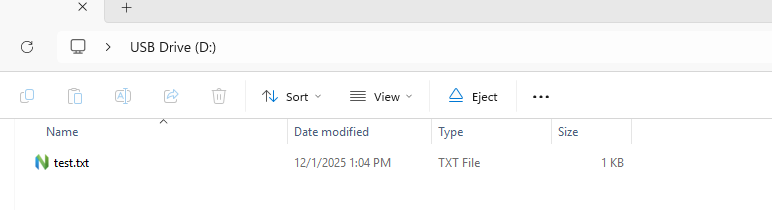
\includegraphics[width=\columnwidth]{accessible_again.png} \caption{Drive can
be accessed again after entering recovery key.} \label{fig:accessible_again}
\end{figure}

\section{Open Research Challenges} 

Due to the potential for destructive disk writes
on boot drives, the experimental program was installed on a computer with a
minimal Windows 11 operating system (version: 25H2). If there is interest in recreating the
experiment. It is highly recommended to use a device that does not have
important data located on the boot drive or to use a virtual machine instead. 

For the experiment to test out the integrity of BitSaver, two 16 GB USB drives
(identical to the ones used during methodology), a 500 GB solid state drive, and a 256 GB non-volatile memory express (NVME),
each with unique BitLocker recovery keys and encryption, were used. For the 500 GB and 256 GB devices, a test on whether or not
an operating system drive can be restored was also added. 

Firstly, all devices had filler data stored on them. Then, BitLocker was turned on for all four individual devices. Afterwards,
all four devices had their BitLocker partitions deleted through DiskPart.
BitSaver will attempt to restore BitLocker functionality to each device
individually. If the device does not seem to respond to the fix, a manual removal and reconnection will be applied
due to occasional read issues from the intermediate reading device or unregistered, modified partition tables.

For each device, several metrics were measured: the type of drive (data or OS),
whether or not the data was recovered, capacity of the disk in bytes, number of
LBA sectors, and logical sector size. These will be used to find out
how effective the program is at restoring BitLocker functionality on various
types of drives and storage sizes.

\section{My Solution}

\subsection{16 GB USB Drive, NTFS/FAT32, Data Only}

The 16 GB USB had a total of 15,728,640,512 Bytes. The device only had a data partition (FAT32 and NTFS) for the entirety of the drive. The disk had
a count of 3,072,001 LBA sectors and a sector size of 512. After the operation, the data was recovered after entering the BitLocker password.
The results worked for both NTFS and FAT32 drives. Interestingly, rewriting the drive as either FAT32 or NTFS worked despite the drive's initial type. However, this will not work
if certain files on the drive are larger than 4 GB due to FAT32's file size limit. Alternatively, NTFS supports up to 4 EB (exabytes) for each file.

\subsection{256 GB NVME, NTFS/FAT32, Data Only}

The 256 GB NVME had a total of 250,051,221,504 Bytes. The device only had a data partition (FAT32 or NTFS) for the entirety of the drive. The disk had
a count of 488,381,292 LBA sectors and a sector size of 512. After the operation, the disk originally was
not reading. However, after a reconnect, the testing operating system recognized the disk's new properties. The data was then recovered after entering the BitLocker password.
The results worked for both NTFS and FAT32 drives. Similar to the previous experiment, partitioning the drive as FAT32 or NTFS worked.

\subsection{256 GB NVME, NTFS, OS Drive}

The 256 GB NVME had a total of 250,051,221,504 Bytes. The device had an operating system partition (Windows 11) in the middle of the drive with a System EFI partition on its
left and a recovery partition on its right. The disk had a count of 488,381,292 LBA sectors and a sector size of 512. After the operation, the disk was not reading. However,
even after the reconnect, the data was not recovered. Instead, the operating system interpretted the 
the partition as RAW. Thus, BitSaver was unable to recover data on this drive.

\subsection{500 GB SSD, NTFS/FAT32, Data Only}

The 500 GB SSD had a total of 500,102,443,008 Bytes. The device only had a data partition (FAT32 or NTFS) for the entirety of the drive. The disk had
a count of 976,762,584 LBA sectors and a sector size of 512. After the operation, the disk originally was
not reading. However, after a reconnect, the testing operating system recognized the disk's new properties. The data was recovered after entering the BitLocker password.
The results worked for both NTFS and FAT32 drives. 

\subsection{500 GB SSD, NTFS, OS Drive}

The 500 GB SSD had a total of 500,102,443,008 Bytes. The device had an operating system partition (Windows 11) in the middle of the drive with a System EFI partition on its
left and a recovery partition on its right. The disk had a count of 976,762,584 LBA sectors and a sector size of 512. After the operation, the disk was not reading. However,
even after the reconnect, the data was not recovered. Instead, the operating system interpretted the 
the partition as RAW. Thus, BitSaver was unable to recover data on this drive.


\section{Conclusions}\label{conclusions} 


\subsection{Findings} 

The program worked well over all the data only drives, which are the most
common drives that suspects can encrypt on-the-fly. In all three experiments
considering data only drives, BitSaver was able to recover the data on all of
them. Some, however, required a reconnect for the testing operating system to
register the drive's new partition table. In addition, it was discovered that FAT32 drives
could be rewritten as NTFS drives and vice versa for this experiment. This is
likely due to the fact that the FAT32 file systems can be read by all operating
systems. However, due to the limitations of the FAT32 system in terms of file
sizes, it is not recommended to try and convert a drive to a different file
system than its original system for risk of data loss. Luckily, the program can rewrite file system
types. If FAT32 does not work for a system, a user may possibly run the program
again and select NTFS instead, which should prevent any data loss.

However, BitSaver did not work for any of the OS drive experiments. Every
experiment resulted in a RAW partition in Disk Manager. Considering that the disk no longer
recognizes the last partition and the first partition (recovery partition and
EFI System partition, respectively), the program likely still needs to account
for partitions that surround the BitLocker partition. In the future, the program should ignore
partitions that are not within the BitLocker scope in order to potentially be compatible with 
BitLocker OS drives.

Overall, the size of a drive is demonstrated to not deter BitSaver's ability to recover 
BitLocker functionality even after an overrided partition deletion through.
The only barrier to the program's effectiveness is whether the drive
is an OS drive or a data drive (which means if there are more partitions on the drive than just the BitLocker partition).

\subsection{Closing Remarks} 
In summary, BitLocker as a technology, though intended to secure data for enterprise and privacy reasons, has become a barrier for
law enforcement and people involved in digital forensics. Even worse, disk partitions with BitLocker encryption can be manually deleted,
which causes standard data reading techniques to be ineffective in reading potentially important data off a suspect's devices. 
Thus, suspects can take advantage of these operations and obscure important
pieces of evidence from law enforcement and even maliciously recover the data at a future date. BitSaver was made to solve
this problem. Through only open source and free software, BitSaver is a program that automatically detects BitLocker partitions
and attempt to rewrite partition tables in order to restore BitLocker functionality on an otherwise unreadable disk. Though there are many commerically avaiable products,
most of the products require money and do not provide free help. For the processes that do teach users how to write their own partition tables, the processes are complicated and not simple for the average user.
Making mistakes while following these sensitive instructions can lead to catastrophic, permanent data loss. Through understanding the structure of file systems and disks, BitSaver identifies BitLocker sectors and safely writes new partition tables
to reestablish deleted partitions and restore the disk's ability to be interpretted. The results indicate great success with restoring
data drives and no success with os drives. However, as the program is still in development, future changes can be applied to fix this issue.

\subsection{Future Plans}

In the future, the project would like to directly explore creating its own
MBR writing component without the use of third-party tools like Runtime
Software's DriveDoppel. There is ground work laid out already on writing
disk partition tables through hexdumps and modifying a disk on the system
level. However, this capability was not explorered in this paper. In addition,
the project would like to explore converting the CLI-based operations into
Application Programming Interface based operations or Graphical User Interface based operations.
However, for the current project
scope, the CLI is believed to be sufficient to demonstrate a proof of concept. Furthermore, BitSaver currently cannot restore
OS drives. However, this can be remedied in the future given the critical results provided by this paper.
Allowing the user to select partitions within a drive potentially would allow for the restoration
to work on a partition level without affecting other partitions (similar to DiskPart). 
Thus, deeper menus to look into partitions would be a necessary future implementation.

\begin{thebibliography}{00} \raggedright 
	\bibitem{b1} “Bitlocker data
	recovery.” Accessed: Dec. 12, 2025. [Online]. Available:
	https://www.runtime.org/bitlocker-data-recovery.htm 
	\bibitem{b2} N.
	Bauer, “How to recover data from a deleted, BitLocker enabled
	partition?,” NORMAN BAUER. Accessed: Dec. 12, 2025. [Online].
	Available:
	https://www.normanbauer.com/2013/07/25/how-to-recover-data-from-a-deleted-bitlocker-enabled-partition/
	\bibitem{b3} Finley and Jaden, “Restore RAW BitLocker Partitions with
	BitLocker Repair Tool,” EaseUS, Dec. 12, 2025. Accessed: Dec. 12, 2025.
	[Online]. Available:
	https://www.easeus.com/data-recovery-solution/restore-file-from-raw-bitlocker-partition.html
	\bibitem{b4} Y. Zhang, “[Solved] How to Recover Deleted or Lost
	BitLocker Partition?,” M3 Software, Aug. 19, 2024. Accessed: Dec. 12,
	2025. [Online]. Available:
	https://www.m3datarecovery.com/bitlocker-drive-data-recovery/recover-deleted-lost-bitlocker-encrypted-partition.html
	\bibitem{b5} B. Hayes, “The Impact of Data Encryption on Digital
	Forensics,” North Forensics. Accessed: Dec. 12, 2025. [Online].
	Available:
	https://www.northforensics.com/post/the-impact-of-data-encryption-on-digital-forensics
	\bibitem{b6} “DiskExplorer — Disk Editor — Data Recovery.” Accessed:
	Dec. 12, 2025. [Online]. Available:
	https://www.runtime.org/diskexplorer.htm\ 
	\bibitem{b7} “DriveDoppel,” Doppel Your Drive for Backup or Data Recovery. Accessed: Dec. 15, 2025. [Online]. Available: https://www.runtime.org/drivedoppel.htm
  




\end{thebibliography}

	\vspace{12pt}

	\end{document}
